\section{Causal Framework}
\label{sec:causal-methodology}
\subsection{Causal Diagram and Variable Definitions}

We model the relationships between article content, sentiment, and ideology using the causal diagram in Figure~\ref{fig:causal_diagram}, which formalizes our assumptions about the data-generating process and determines which variables must be controlled for to obtain unbiased causal estimates.

We define the following variables:
\begin{itemize}
    \item $X$: (text) the full article text parsed from the publishing source.
    \item $T$: (topic tags) AllSidesV2 topic tags (e.g.\ Politics, Government Efficiency, Foreign Affairs).
    \item $F$: (sentiment) sentiment toward each topic, inferred from article text using an LLM.
    \item $Y$: (perceived ideology) the ideology label assigned by the annotator (human and LLM).
\end{itemize}

\begin{figure}[h]
    \centering
    \begin{subfigure}{0.45\textwidth}
        \centering
        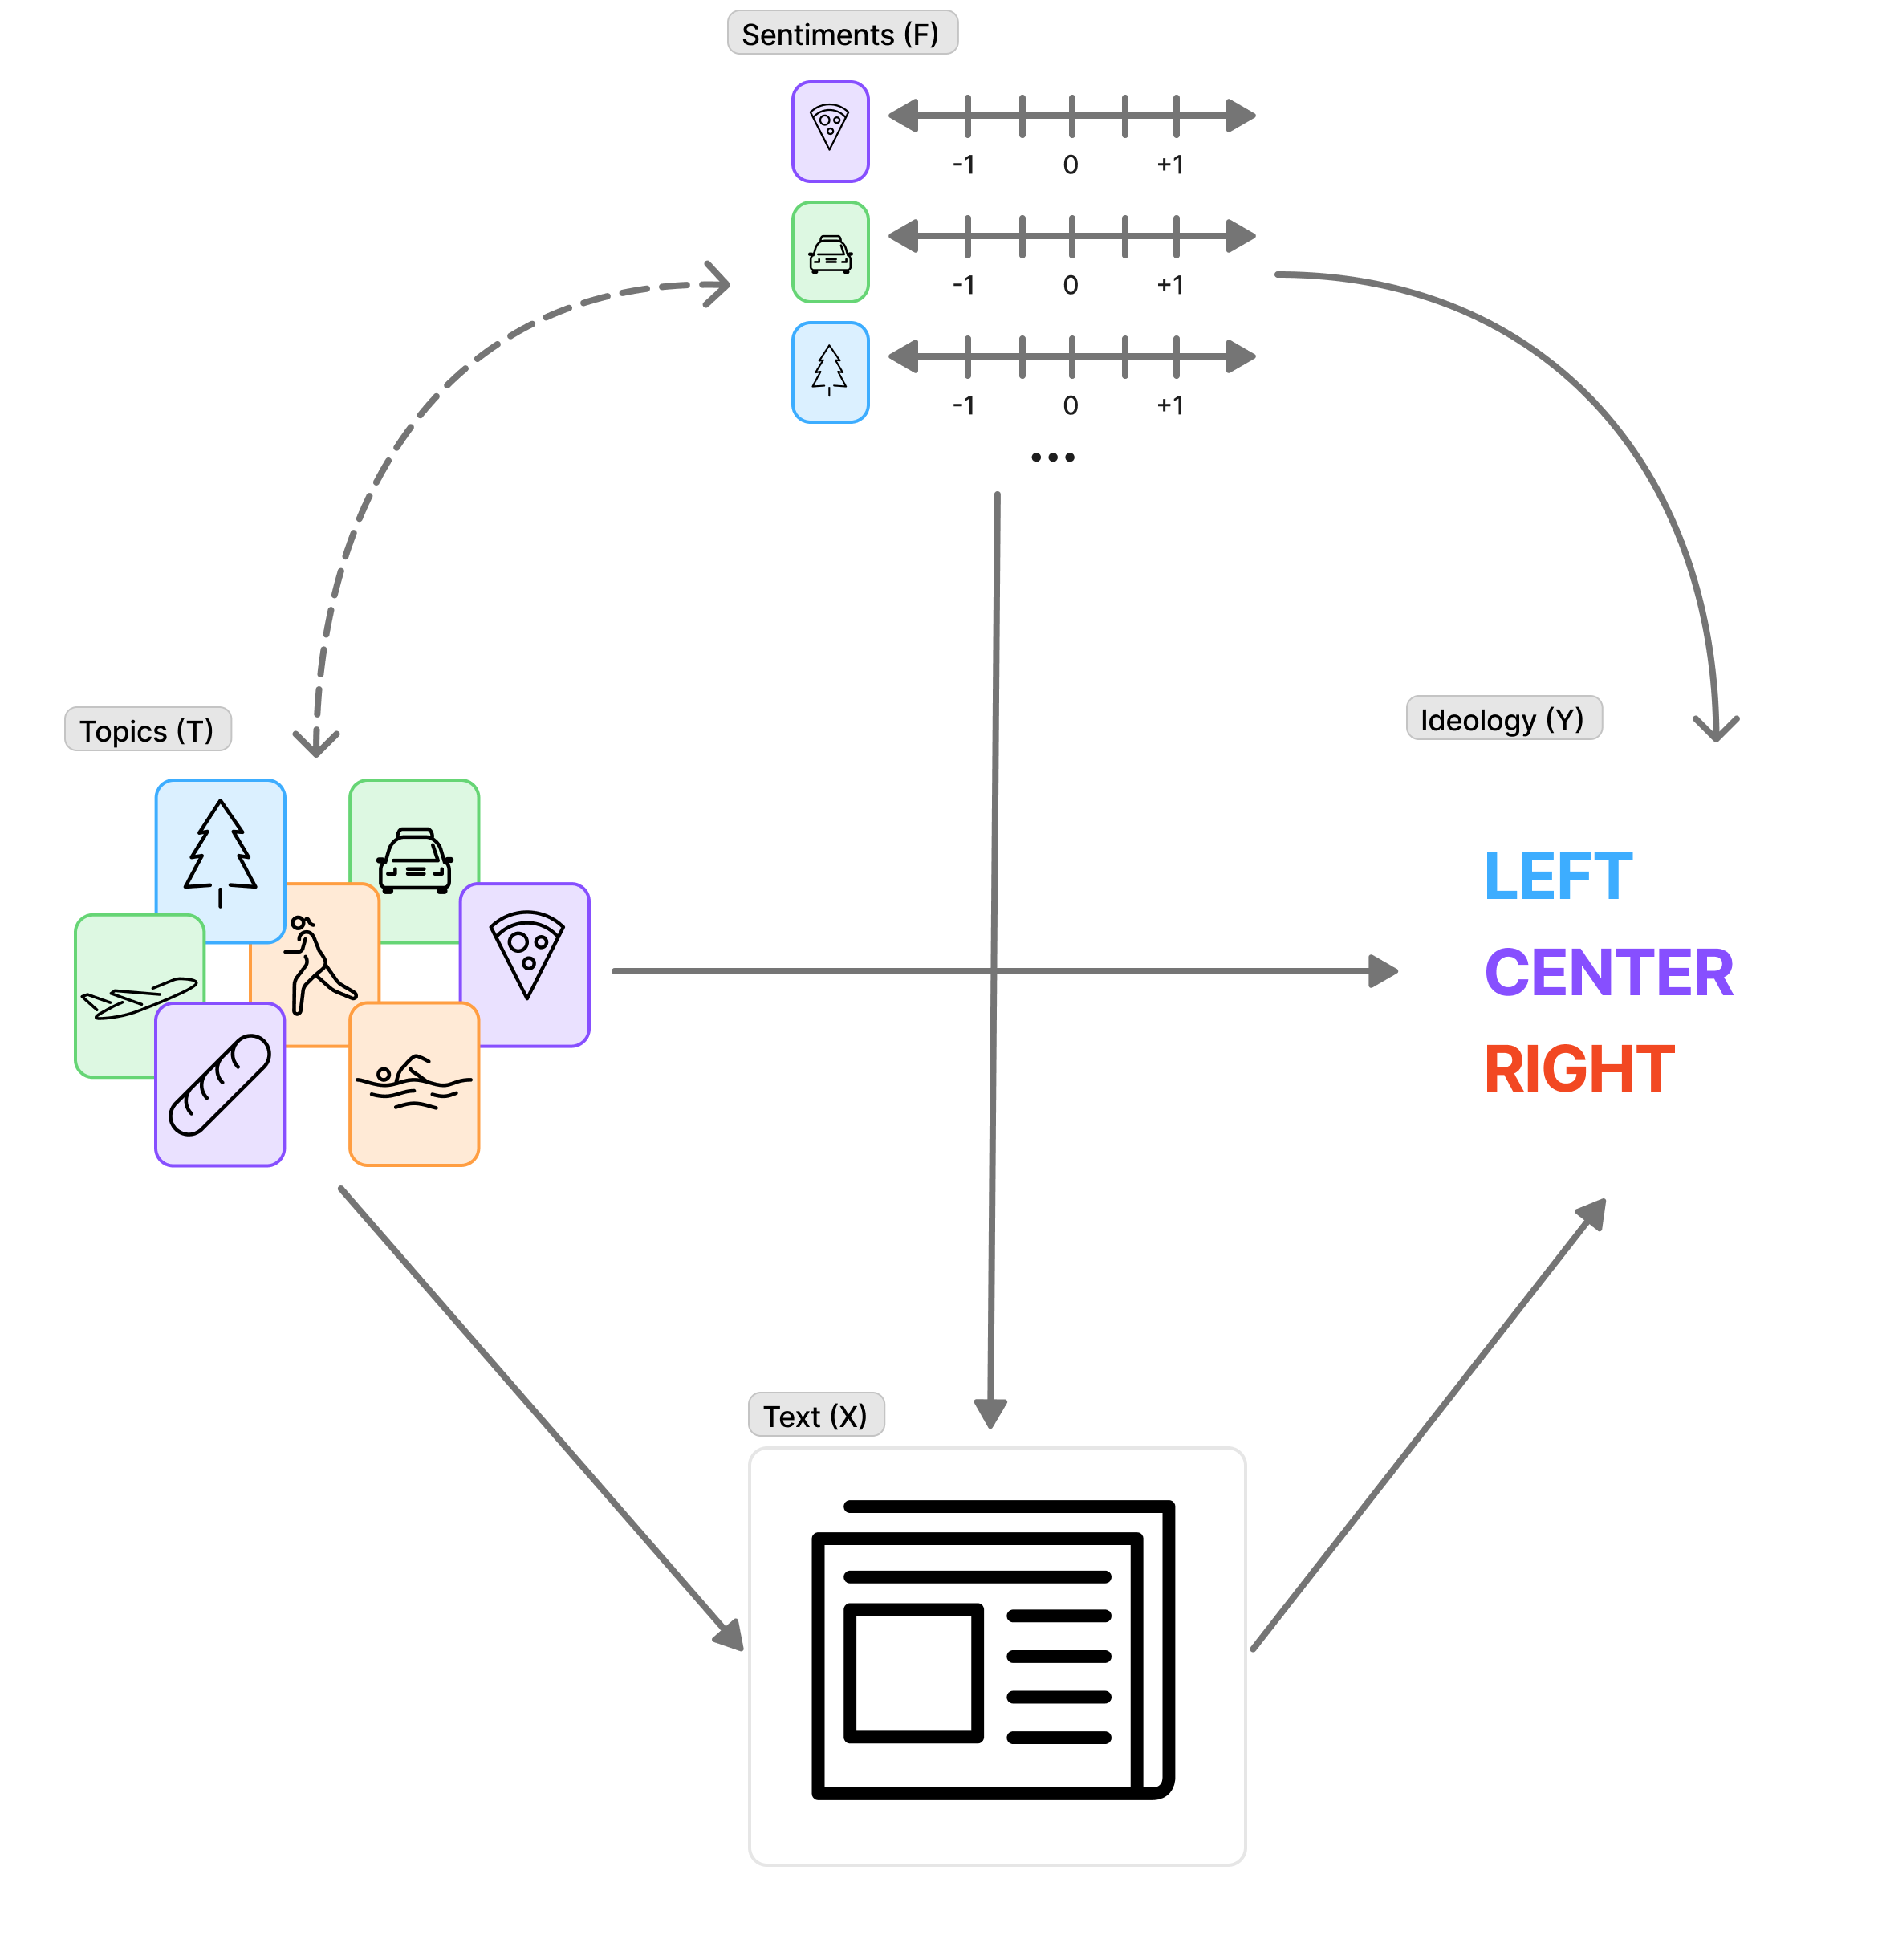
\includegraphics[width=\textwidth]{sections/images/causal_diagram.png}
        \subcaption{Illustrated representation}
    \end{subfigure}
    \hfill
    \begin{subfigure}{0.45\textwidth}
        \centering
        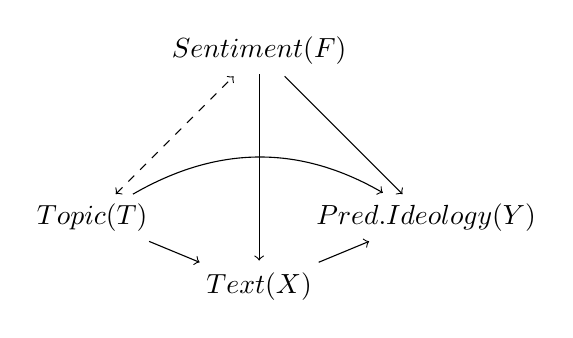
\begin{tikzpicture}[->,shorten >=1pt,auto,node distance=3cm]
          \tikzstyle{every state}=[]

          \node(text) {$\text{Text } (X)$};
          \node(sentiment) [above of=text] {$\text{Sentiment } (F)$} edge [->] (text);
          \node(ideology) [below right of=sentiment] {$\text{Pred. Ideology } (Y)$} edge [<-] (sentiment) edge [<-] (text);
          \node(topic) [below left of=sentiment] {$\text{Topic } (T)$} edge [->] (text) edge [->, bend left] (ideology) edge [<->, dashed] (sentiment);
        \end{tikzpicture}
        \subcaption{Simplified graph}
    \end{subfigure}
    \caption{Complete causal diagram for article ideology classification. The topics serve as indicator variables to represent the presence or absence of specific topics. Each sentiment is a continuous variable and is topic-specific. The predicted ideology is a categorical variable. Each article may have multiple topics. Note, we do not include article text in our investigations.}
    \label{fig:causal_diagram}
\end{figure}

Each arrow represents a hypothesized causal direction. The arrow from $Y$ to $X$ reflects that ideology shapes article content and framing. The arrow from $F$ to $X$ reflects that sentiment toward a topic influences how that topic is discussed. The bidirectional dashed arrow between $T$ and $F$ captures the mutual relationship between topics and sentiment: certain topics tend to evoke particular sentiments, while prevailing sentiment patterns influence which topics receive coverage. The bidirectional edge is the model's way of acknowledging that the existence of a topic in a given article and the sentiment expressed toward that topic are jointly shaped by upstream factors (the time period the article was written in, the publishing outlet's editorial stance, broader social and political conditions) that are not directly modeled here. Rather than commit to a single direction, we represent the dependence as bidirectional.

In practice, each node expands into many variables. Figure~\ref{fig:causal3} illustrates this: each sentiment node $F$ corresponds to a distinct topic, and sentiment toward one topic ($F_T$, the treatment) may influence sentiment toward other topics ($F_{M_1}, F_{M_2}, \ldots$, the mediators), which in turn affect ideology classification $Y$. The structural relationships \textit{between} variable types remain as in Figure~\ref{fig:causal_diagram}; what changes is the dimensionality \textit{within} each node.

\begin{figure}[h!]
  \centering
  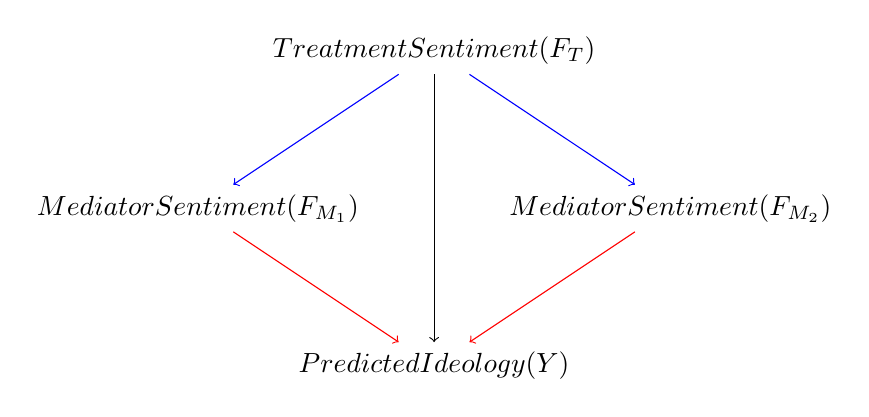
\begin{tikzpicture}[->,auto]
    % Top row: the three F's
    \node (FT)   at (0,0)   {$\text{Treatment Sentiment } (F_{T})$};
    \node (FM1)  at (-3,-2)   {$\text{Mediator Sentiment } (F_{M_1})$};
    \node (FM2)  at (3,-2)   {$\text{Mediator Sentiment } (F_{M_2})$};

    % Bottom row: the three observed variables
    % \node (Xabs) at (1.5,-2)  {$X$};
    \node (Y)    at (0,-4)  {$\text{Predicted Ideology } (Y)$};
    % \node (TT)    at (-2,1)  {$T_{T}$};
    % \node (TM1)    at (-2,0)  {$T_{M_1}$};


    % Edges from F_T
    \draw[->]           (FT) -- (Y);
    % \draw[->]  (FT) -- (Xabs);
    % \draw[<->, dashed]  (FT) -- (TT);

    % Edges from X_abs and T to Y
    % \draw[->]  (Xabs) -- (Y);
    % \draw[->]  (TT) to (Y);
    % \draw[->]  (TM1) to (Y);

    % % Edges from TT and TM1 to X_abs
    % \draw[->]  (TT) to (Xabs);
    % \draw[->]  (TM1) to (Xabs);

    % Edges for F_{M_1}
    \draw[->, red]             (FM1) -- (Y);
    % \draw[->, red]    (FM1) -- (Xabs);
    % \draw[<->, dashed, red]    (FM1) -- (TM1);
    \draw[<-, blue]            (FM1) -- (FT);

    % % Edges for F_{M_2}
    \draw[->, red]             (FM2) -- (Y);
    % \draw[->, red]    (FM2) -- (Xabs);
    % \draw[<->, dashed, red]    (FM2) -- (TM1);
    \draw[<-, blue] (FM2) to (FT);
  \end{tikzpicture}
  \caption{Expanded setup: sentiment variables as mediators. Blue arrows show treatment-to-mediator paths; red shows mediator-to-outcome paths. For our investigations, we focus on a single treatment-mediator pair at a time, but the same framework can be extended to support multiple mediators. We omit the text variable $X$ and the topic variable $T$ for visual clarity, as they do not directly participate in the causal relationships of interest.}
  \label{fig:causal3}
\end{figure}

The roles of each variable in the estimation framework are:

\paragraph{Treatment Variable ($F_T$):} Sentiment toward a specific topic of interest (e.g., sentiment toward ``Immigration'' or ``Healthcare''). This is the variable whose causal effect on ideology we seek to estimate.

\paragraph{Outcome Variable ($Y$):} The ideology label (Left/Center/Right) assigned to the article.

\paragraph{Mediator Variables ($F_{M_1}, F_{M_2}, \ldots$):} Sentiment toward all other topics present in the article. These lie on the causal pathway between treatment sentiment and ideology: sentiment toward one topic may influence sentiment toward related topics, which in turn affects ideology classification. Blue arrows in Figure~\ref{fig:causal3} show these paths.

\paragraph{Confounder Variables:} $T$ (topic presence) is the primary confounder, since the presence of a topic influences both sentiment toward it and the overall ideological character of the article. $X$ (text content) acts as a collider, influenced by both sentiment and ideology.

We restrict the analysis to articles containing the treatment topic, preventing invalid comparisons between articles that discuss a topic and those that do not. This design supports estimation of Average Treatment Effects (ATE), Conditional Average Treatment Effects (CATE), Natural Direct Effects (NDE), and Natural Indirect Effects (NIE).

\subsection{Data Collection}

\paragraph{Test-set-only restriction.} A central design choice for the entire causal analysis in this chapter is that all estimates are computed exclusively on the held-out test split of AllSidesV2 Media, with no overlap whatsoever with any classifier's fine-tuning or continued-pre-training data. This restriction is not a routine evaluation hygiene note: it is load-bearing for the interpretation of every causal estimate that follows. If the analysis were run on data that the classifiers had been trained on, the estimated causal pathways from sentiment and topic to ideology could simply reflect memorized training-set associations rather than learned generalizations, and a model that had memorized a spurious sentiment--ideology link in its training set would look identical under causal probing to a model that had learned a real one. By restricting the analysis to test-set articles, we ensure that any causal pathway we measure for a given annotator reflects how that annotator generalizes to unseen articles, not how it remembers its training data, which is the property we actually care about when comparing human, fine-tuned, and zero-shot annotators.

We use the AllSidesV2 dataset described in Section~\ref{sec:dataset}. All causal analyses are performed on the test set of the AllSidesV2 Media split (9,830 articles) to ensure fair comparison across annotation sources. To extract sentiment variables ($F$), we apply a two-step process to the full article text ($X$):

\begin{enumerate}
\item \textbf{Entity and Sentiment Analysis:} Named entities and key concepts are extracted from the corpus. The \texttt{llama-3.3-70b-versatile} model assigns sentiment polarity to each entity on a continuous scale from $-1.0$ (strongly negative) to $+1.0$ (strongly positive). This model was chosen for its sensitivity to contextual nuances compared to smaller alternatives.

\item \textbf{Entity-to-Topic Association:} The \texttt{llama3-70b-8192} model quantifies how strongly each extracted entity relates to predefined AllSides topic tags. The model avoids spurious correlations; for example, correctly distinguishing between terrorism as a broad concept and specific incidents like the 2019 Christchurch shooting when assigning the entity ``shooting'' to a topic. Entity sentiment scores are then aggregated by topic tag to produce a per-topic sentiment profile for each article.
\end{enumerate}

\subsection{Experimental Design}
\label{sec:experimental-design}



We perform all analyses on the test set of the AllSidesV2 Media split to ensure fair comparison across annotation sources. To identify the topical structure of this set, we apply the Louvain community detection algorithm to a co-occurrence graph of topic tags, where nodes are tags and edge weights reflect how often two tags appear together in the same article. Self-loops allow single-tag articles to form their own communities. This yields a modularity score of 0.498 across 12 communities, with community sizes ranging from 1 to 199 tags.

\begin{figure}[h]
  \centering
  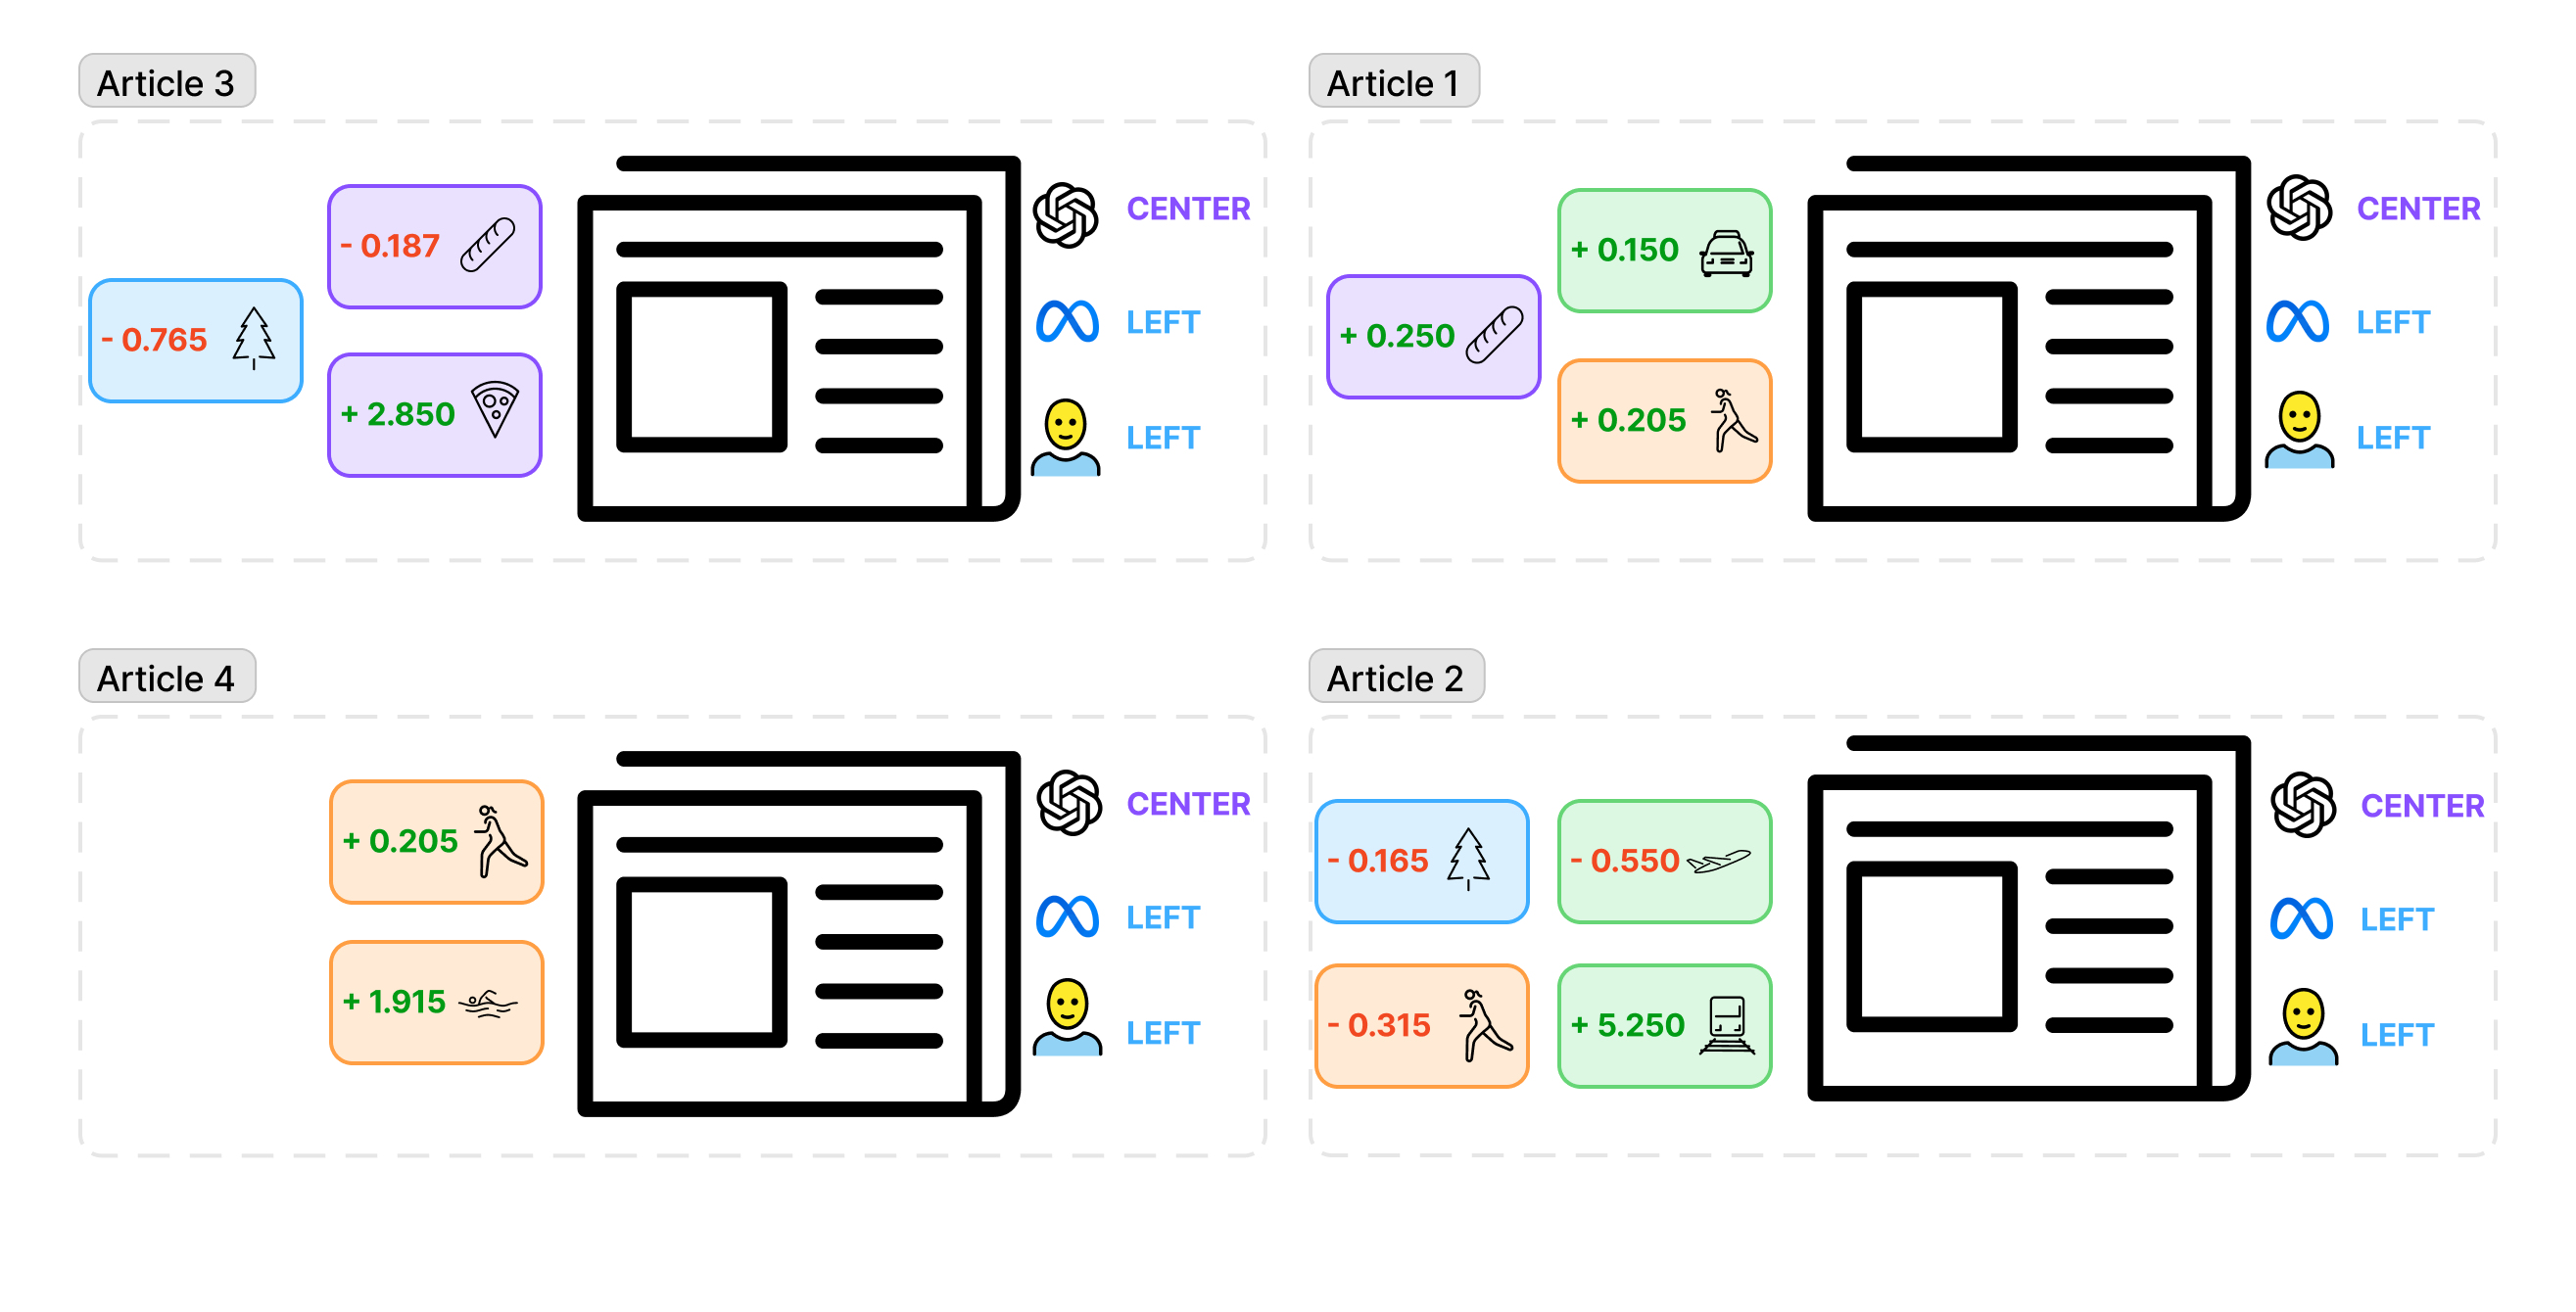
\includegraphics[width=0.8\textwidth]{sections/images/articles.png}
  \caption{Articles with predicted ideologies, topics, sentiments, and topic clustering. To the left of each article we see coloured boxes that represent a topic and topic-specific sentiment. The distinct colours represent distinct communities. To the right we see different annotators and their predicted ideologies for the article.}
  \label{fig:articles}
\end{figure}

The final representation of an article can be seen in Figure~\ref{fig:articles}. We note that the presence of multiple topics and sentiments within a single article creates a complex web of potential causal pathways to ideology, which motivates our use of community aggregation to disentangle direct and indirect effects at a higher level. 

\begin{table}[h]
    \centering
    \begin{minipage}{0.45\textwidth}
        \centering
        \small
        \begin{tabular}{lcc}
        \toprule
        \textbf{Comm.} & \textbf{Articles}  & \textbf{Theme} \\
        \midrule
        11 & 772  & Trump Administration \\
        4 & 229  & Media and Big Tech \\
        1 & 220 & Elections and Campaigns \\
        7 & 218  & Foreign Policy \\
        5 & 193  & Policing and Social Justice \\
        \bottomrule
        \end{tabular}
    \end{minipage}
    \hfill
    \begin{minipage}{0.45\textwidth}
        \centering
        \small
        \begin{tabular}{lcc}
        \toprule
        \textbf{Topic Tag} & \textbf{Articles} & \textbf{Comm.} \\
        \midrule
        Politics & 594 & 11 \\
        Donald Trump & 233 & 11 \\
        world & 503 & 9 \\
        elections & 451 & 1 \\
        white\_house & 444 & 11 \\
        \bottomrule
        \end{tabular}
    \end{minipage}
    \caption{Top five communities and topic tags in the AllsidesV2 media split test set. Total article count is 9,830. The full community structure with all 15 communities and their constituent topics is provided in Appendix~\ref{appendix:community-structure}.}
    \label{tab:topical-summary}
\end{table}

%\begin{figure}[h!]
%    \centering
%    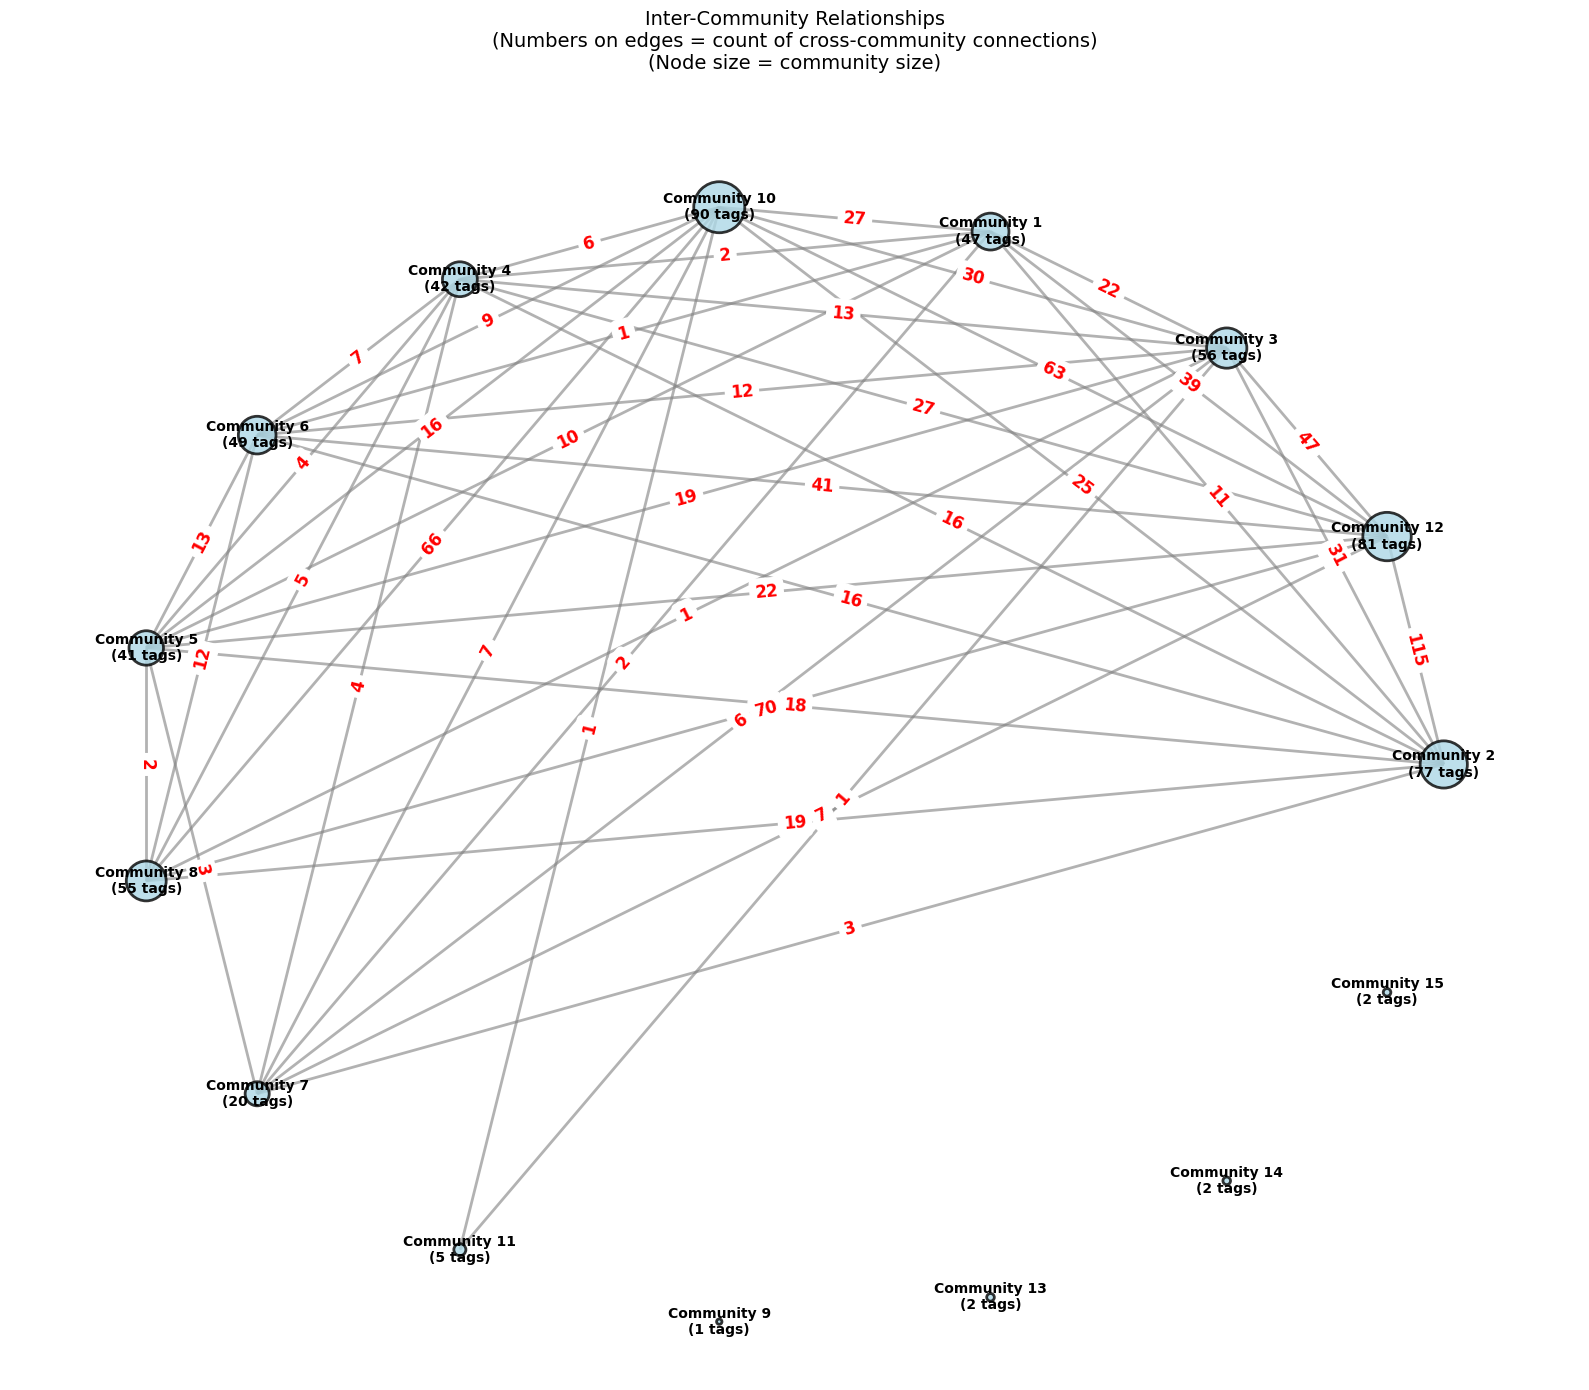
\includegraphics[width=0.7\textwidth]{sections/images/louvain_communities.png}
%    \caption{Louvain community detection on the topic tag co-occurrence graph for the top five tags.}
%    \label{fig:louvain}
%\end{figure}

Our primary experiments operate at the community level, where aggregating semantically related topics yields larger sample sizes and more robust causal estimates. We estimate ATEs for each community's aggregate sentiment on ideology classification, and conduct mediation analysis to test whether institutional political topics (Community 3) systematically mediate the effects of Trump Administration sentiment (Community 11) on ideology. We estimate CATEs for different combinations of these community-level sentiment variables, testing whether the relationship between individual figures and institutional framing reflects a stable structural pattern.

For completeness, we also perform topic-level mediation analysis on the two most prominent individual tags (top five topics can be seen in Table~\ref{tab:topical-summary}), \textit{donald\_trump} and \textit{politics}, examining their bidirectional relationship in shaping ideology classification. We test two competing hypotheses: (1) Trump sentiment drives general political sentiment, which then shapes ideology; versus (2) broader political sentiment shapes Trump-specific framing, with Trump sentiment mediating the path to ideology. We use NIE/NDE decomposition and bidirectional mediation to determine the dominant pathway.

\subsection{Annotation Paradigms}
\label{sec:annotation-paradigms}

All experiments are conducted across five annotation paradigms. \textbf{Human annotations} are the manual ideology labels from AllSides, serving as our reference point. We note explicitly that the human-baseline portion of this thesis was conducted under an informal study design (uncompensated annotators socially acquainted with the author, ideologically homogeneous pool, self-administered protocol over a one-month window; see Appendix~\ref{sec:appendix-human-tests} for the full disclosure of agreement scores and protocol issues). The human paradigm should therefore be read as an informal lay-annotator reference rather than as fully validated expert ground truth, and the cross-paradigm divergences we report below should be interpreted with this caveat in mind. \textbf{Fine-tuned RoBERTa} uses predictions from the best-performing domain-adapted classifier from Section~\ref{sec:continued-pretraining}. \textbf{GPT-4o-mini (baseline)} provides zero-shot predictions from GPT-4o-mini without task-specific fine-tuning. \textbf{Fine-tuned GPT-4o-mini} uses predictions from the fine-tuned GPT model described in Section~\ref{sec:llm-finetuning}. Finally, \textbf{Llama-3.3-70B} provides zero-shot predictions from Meta's Llama-3.3-70B-versatile model, included to test whether causal patterns generalize across LLM families or are specific to the GPT architecture.

Table~\ref{tab:llm-causal-performance} summarizes the classification performance of each paradigm on the AllSidesV2 test set.

\begin{table}[h]
    \centering
    \begin{tabular}{lc}
    \toprule
    \textbf{Paradigm} & \textbf{F1-Macro} \\
    \midrule
    Fine-tuned GPT-4o-mini & 72.48 \\
    Llama-3.3-70B & 54.61 \\
    GPT-4o-mini (baseline) & 50.07 \\
    Fine-tuned RoBERTa & 62.19 \\
    \bottomrule
    \end{tabular}
    \caption{Machine classification performance on AllSidesV2 test set.}
    \label{tab:llm-causal-performance}
\end{table}

This five-way comparison is structured so that each pairwise contrast isolates a distinct question about how annotation methodology shapes downstream causal estimates. \textbf{Human vs.\ Fine-tuned RoBERTa} isolates the effect of supervised encoder fine-tuning under controlled (non-LLM) pretraining: both pipelines see the same text, but RoBERTa replaces human judgment with a learned classifier whose pretraining is fully transparent. \textbf{GPT-4o-mini (baseline) vs.\ Fine-tuned GPT-4o-mini} isolates the effect of task-specific fine-tuning alone, holding the underlying LLM architecture and pretraining fixed; any divergence in causal structure between these two paradigms is attributable specifically to the fine-tuning step. \textbf{Llama-3.3-70B vs.\ GPT-4o-mini (baseline)} isolates LLM-family effects, holding the absence of task-specific fine-tuning fixed and varying only the underlying model family. Finally, \textbf{the full five-way comparison} isolates the paradigm-dependence of the causal estimates themselves: whether the same article-level sentiment--ideology pathway is recovered consistently regardless of how the labels were produced, or whether annotation methodology alone is enough to change the answer.

\subsubsection{Double Machine Learning}
\label{sec:dml}

Ordinary regression of $Y$ on $F_T$ is biased when confounders $W$ predict both $F_T$ and $Y$. For example, articles from right-leaning outlets may mention the FBI more often \emph{and} receive right-leaning labels, creating a spurious positive correlation between FBI sentiment and ideology that is driven by outlet identity rather than sentiment itself.

We use Double Machine Learning (DML; see Section~\ref{sec:dml-related-work} for the conceptual introduction) to address this. Concretely, in the first stage we fit $\hat{g}(W)$ to predict $Y$ from $W$ and $\hat{m}(W)$ to predict $F_T$ from $W$, yielding residuals $\tilde{Y} = Y - \hat{g}(W)$ and $\tilde{F}_T = F_T - \hat{m}(W)$. In the second stage we regress $\tilde{Y}$ on $\tilde{F}_T$ to obtain the ATE. The 1691 AllSides topic-presence indicators serve as $W$. \authortodo{Add a diagram illustrating the two-stage residualization process.}

After residualization, both $Y$ and $F_T$ have had their confounder-explained variation removed, so the final regression captures only the direct sentiment--ideology relationship that topic presence cannot explain. We implement DML via EconML's \texttt{LinearDML} estimator~\citep{econml} with Random Forest base learners (\num{200} trees, maximum depth~5) and $k = 5$-fold cross-fitting, and extend it with bootstrap-based confidence intervals for mediation effect decomposition.

The ATE is interpreted as: ``holding topic-presence composition constant, a one-unit increase in $F_T$ shifts the expected ideology label by $\widehat{\text{ATE}}$ units on the $[0,2]$ scale.''

\subsubsection{Mediation Analysis}
\label{sec:mediation-design}

The ATE tells us \emph{whether} a topic's sentiment shifts ideology predictions, but not \emph{through which pathways}. As Figure~\ref{fig:articles} illustrates, each article carries sentiment scores for multiple topics, and these topics cluster into communities (indicated by color). When an article discusses topics from several communities simultaneously, a natural question arises: does sentiment toward one community's topics affect ideology prediction directly, or does it do so indirectly by first shifting sentiment toward another community's topics?

Consider the Khalil arrest coverage in Table~\ref{fig:khalil}. AP and Fox News both tag the article with the same topics (Pro-Palestine Protests, Donald Trump, Israel, Deportations) yet their sentiment toward these topics diverges sharply. A mediation analysis asks: does pro-Palestine sentiment shift the ideology prediction directly (a \textbf{direct effect}), or does it do so by also shifting sentiment toward deportation policy, which in turn influences the ideology label (an \textbf{indirect effect})? Distinguishing these pathways reveals whether ideology classifiers respond to isolated topic framing or to correlated sentiment patterns across topics.

Formally, the Total Effect (TE) decomposes into:

\begin{equation}
  \underbrace{\text{TE}}_{\text{Total}} =
  \underbrace{\text{NDE}}_{\substack{\text{Natural Direct}\\ \text{Effect}}} +
  \underbrace{\text{NIE}}_{\substack{\text{Natural Indirect}\\ \text{Effect}}}
\end{equation}

\begin{itemize}
  \item The \textbf{Natural Direct Effect (NDE)} is the portion of the treatment's influence on ideology that operates independently of the mediator: the effect that remains even if the mediator's sentiment were held fixed.
  \item The \textbf{Natural Indirect Effect (NIE)} captures the portion that routes through the mediator: treatment sentiment shifts the mediator's sentiment ($F_T \to F_M$), which in turn shifts the ideology prediction ($F_M \to Y$).
\end{itemize}

For example, positive Trump sentiment ($F_T$) may incline an article toward positive Politics framing ($F_M$). If positive Politics sentiment then influences the ideology classifier, the NIE captures that indirect path; the NDE captures all remaining direct pathways. In Figure~\ref{fig:articles}, topics sharing the same color belong to the same Louvain community; when we perform community-level mediation (Section~\ref{sec:community-aggregation}), we aggregate all same-colored topics into a single community sentiment score and ask whether one community's aggregate sentiment affects ideology directly or through its influence on another community's sentiment.

We estimate NDE and NIE using nested DML estimators with $B = \num{2000}$ bootstrap iterations for 95\% confidence intervals. Because the TE confidence interval consistently includes zero in our results (see Section~\ref{sec:mediation-results}), we suppress the proportional mediation $(\text{NIE}/\text{TE})$ to avoid division-by-near-zero artifacts.


\begin{figure}[h!]
  \centering
  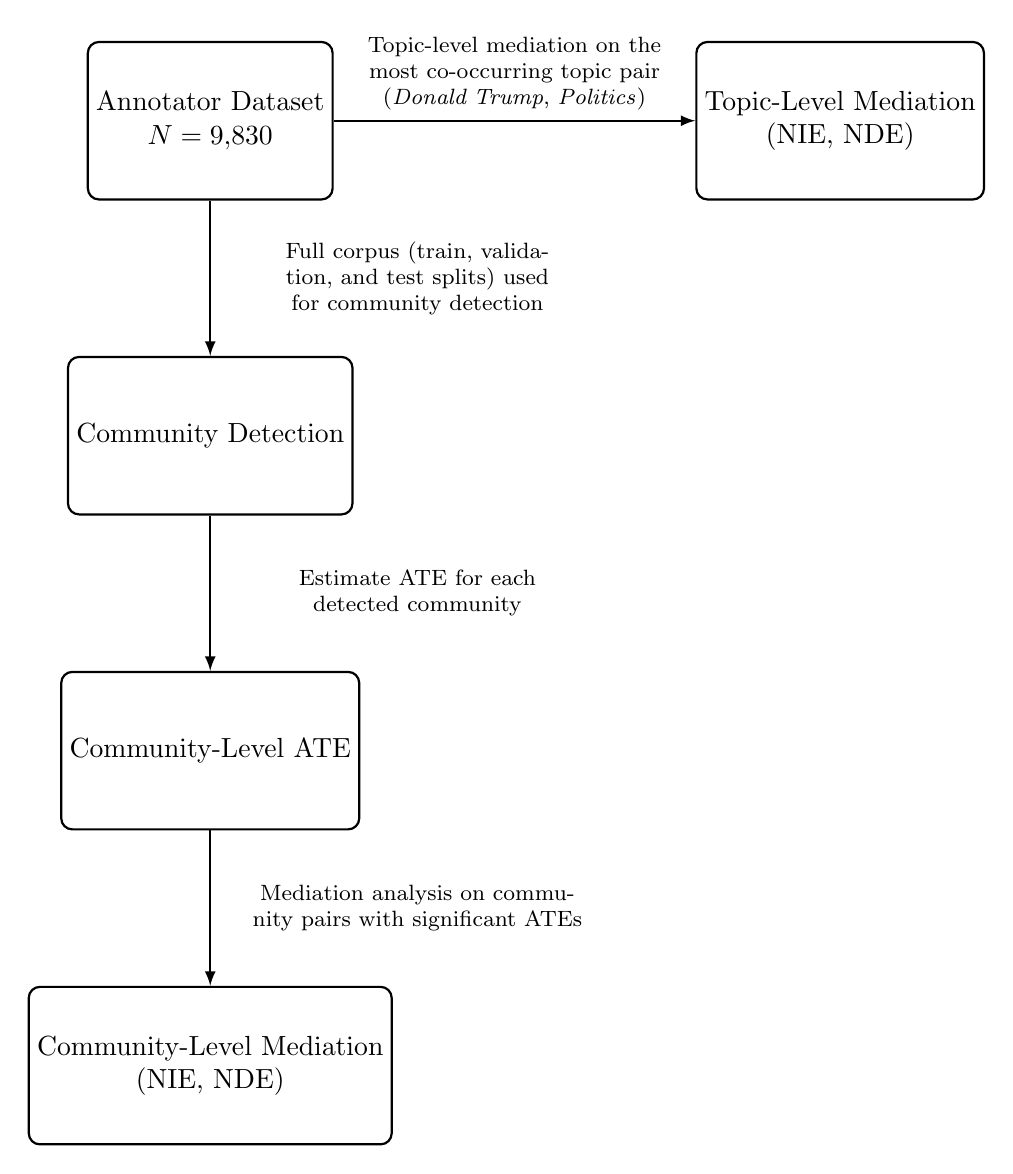
\begin{tikzpicture}[
      >=latex,
      procnode/.style={
          rectangle, rounded corners,
          draw, thick,
          minimum width=2.8cm, minimum height=2cm,
          align=center, inner sep=3pt
      },
      edgelabel/.style={
          font=\footnotesize, align=center
      }
  ]
    % (a) Annotator dataset
    \node[procnode] (a) at (0,0) {Annotator Dataset\\$N = 9{,}830$};

    % (e) Topic-level mediation (to the right of (a))
    \node[procnode] (e) at (8,0) {Topic-Level Mediation\\(NIE, NDE)};

    % (b) Community detection (below (a))
    \node[procnode] (b) at (0,-4) {Community Detection};

    % (c) Community-level ATE (below (b))
    \node[procnode] (c) at (0,-8) {Community-Level ATE};

    % (d) Community-level mediation (below (c))
    \node[procnode] (d) at (0,-12) {Community-Level Mediation\\(NIE, NDE)};

    % Edges
    \draw[->, thick] (a) -- node[edgelabel, above, text width=4.8cm]
        {Topic-level mediation on the most co-occurring topic pair (\textit{Donald Trump}, \textit{Politics})} (e);
    \draw[->, thick] (a) -- node[edgelabel, right, text width=5cm]
        {Full corpus (train, validation, and test splits) used for community detection} (b);
    \draw[->, thick] (b) -- node[edgelabel, right, text width=5cm]
        {Estimate ATE for each detected community} (c);
    \draw[->, thick] (c) -- node[edgelabel, right, text width=5cm]
        {Mediation analysis on community pairs with significant ATEs} (d);
  \end{tikzpicture}
  \caption{Overview of the full experimental procedure of Chapter~\ref{sec:causal-inference}. The annotator dataset feeds two parallel analyses: a community-level pipeline (community detection, followed by ATE estimation and then mediation on community pairs with significant effects) and a topic-level mediation analysis on the most frequently co-occurring topic pair.}
  \label{fig:experimental-procedure}
\end{figure}


\subsubsection{Treatment Encoding and Contrasts}
\label{sec:treatment-encoding}

All analyses use a continuous treatment encoding: the raw sentiment score on the $[-100, +100]$ scale, standardized (zero mean, unit variance) before estimation, so that the ATE represents the effect of a one-standard-deviation increase. This preserves fine-grained variation: a score of $+45$ carries more positive framing than $+1$.

For the mediation analysis, treatment contrasts are evaluated at the interquartile range ($Q25 \to Q75$, primary) and the 10th--90th percentile range ($P10 \to P90$, secondary), computed from the empirical distribution of the continuous treatment score in the filtered subsample. For example, a CATE of $-0.21$ for Left-leaning outlets means that increasing Trump sentiment from $Q25$ to $Q75$ is associated with a $-0.21$ shift in ideology on the $[0,2]$ scale.

\subsubsection{Confounder Dimensionality Reduction}
\label{sec:pca}

The topic-presence indicator matrix $W$ has \num{1691} columns, one per AllSides topic tag. We apply PCA to $W$, retaining components that together explain 95\% of the variance (capped at 50 components). The 95\% threshold is chosen because it preserves the substantive between-topic variation that drives our causal estimates while collapsing the long tail of low-variance dimensions that mostly contribute estimation noise; the 50-component cap is necessary to keep nuisance-model fitting numerically stable in the smaller filtered subsamples used for mediation, where the effective sample size can drop into the low hundreds and an unconstrained PCA expansion would over-parameterize the first-stage models.

Missing topic-presence values are imputed as 0, reflecting the semantic equivalence of ``topic absent'' and ``indicator = 0.'' Sentiment scores for absent topics are similarly imputed as 0 (neutral).

\subsubsection{Multi-Treatment DML}
\label{sec:multi-treatment-design}

While mediation analysis fits one model per topic pair $(F_T, F_M)$, a complementary approach fits a \emph{single} model with all qualifying topic sentiments simultaneously as a treatment matrix $\mathbf{T} \in \mathbb{R}^{N \times k}$. This controls for correlations among sentiments and yields one ATE per topic, interpreted as the effect of that topic's sentiment \emph{holding all other topic sentiments constant}.

\subsection{Community-Level Aggregation}
\label{sec:community-aggregation}

In addition to the topic-level analysis above, we perform a community-level analysis that aggregates sentiments within detected topic communities. The community sentiment $F_C$ is the mean sentiment over member topics present in an article, and equals zero when no member topic appears. Let $\mathbf{F}_C = (F_{C_1}, \ldots, F_{C_L})$ be the community-aggregated treatment matrix. The marginal ATE for each community $C_\ell$ is

\begin{equation}
  ATE_{C_\ell} = E\!\left[\frac{\partial Y}{\partial F_{C_\ell}}\right], \quad \forall\, \ell = 1, \ldots, L,
  \label{eq:ate_comm}
\end{equation}

\noindent estimated via a single \texttt{LinearDML} model with $\mathbf{F}_C$ as the treatment matrix and PCA-reduced topic-presence indicators as confounders. Community-level aggregation increases the number of articles per treatment unit and yields more reliable estimates than topic-level analysis, particularly for topics that individually appear in few articles.

For community-level mediation, we restrict the analysis to articles that contain topics from \emph{both} the treatment community and the mediator community. Returning to Figure~\ref{fig:articles}, this means selecting only articles whose topic tags span at least two community colors, i.e. communities where the treatment community's sentiment and the mediator community's sentiment are both observable. \authortodo{Add community level results when available.}

Sections~\ref{sec:community-level-results} and~\ref{sec:topic-level-results} present the empirical analysis at two levels of granularity. We lead with \emph{community-level} results because they are the more robust analysis: aggregating sentiments within Louvain-detected topic communities pools many low-frequency topics into a smaller number of high-frequency treatments, which increases per-treatment sample size, stabilizes the nuisance-model fits, and supports tighter confidence intervals. The \emph{topic-level} results that follow are presented as a finer-grained robustness check on the same data, asking whether the community-level picture holds when we look at individual topics with much smaller per-treatment $N$.

Figure~\ref{fig:experimental-procedure} summarises the full experimental pipeline of this chapter, showing how the annotator dataset feeds the community-level chain of analyses (community detection, ATE estimation, mediation) and, in parallel, the topic-level mediation analysis on the most frequently co-occurring topic pair.

